\chapter{Results} \label{chap:results}
In this chapter, the obtained results from the defined experiments in section \ref{sec:experiments} are presented. In section \ref{sec:exp_feas} we summarized the results for the feasibility test of a deep-learning based peripheral nerve segmentation.
Section \ref{sec:exp_3dcontext} presents the achieved performances for the defined segmentation metrics for the different neural network architectures with variable access to 3D information.
In section \ref{sec:exp_pp} the results for the impact-study of post-processing applied to the segmentation of the baseline architecture and the best performing 3D architecture, respectively.
Finally, section \ref{sec:exp_evaluation} features the results obtained concerning the inter-rater variability, to which we compare and evaluate our best performing 3D architecture.
The detailed results of the individual experiments can be found in the appendix \ref{app:results}.

\section{Experiment 1: Feasibility} \label{sec:exp_feas} %=======================================================
We successfully trained the baseline architecture on the \gls{mrn} images. In order to gain some insight in the importance of the two input channels (T2 and \gls{ir}), we trained the baseline architecture a total of three times: Once on each channel separately, and once with both of them. The mean and \gls{sd} for each of the training runs are summarized in Table~\ref{tab:results_feasibility}. Figure~\ref{fig:results_boxplot_T2_IR_dice} features a boxplot for the \acrlong{dice}. The training took 3 hours on a NVIDIA Titan Xp for each of the runs.

\begin{table}[htbp]
   \centering
   \caption[Metrics for Baseline with different Input Channels]{Values for \acrlong{dice}, \acrlong{vs} and \acrlong{hd95} for the baseline architecture. The architecture was trained and evaluated on T2-only, IR-only and on the combination of them.}
   \begin{tabular}{l*{4}{l}}
      \toprule
      Cohort	& Channels  & DICE              & VS				& HD95\\
      			&			&					&					& (mm)\\
      \midrule
      Patient   & T2 and IR & $\mathbf{0.704 \pm 0.139}$& $\mathbf{0.882 \pm 0.098}$ & $\mathbf{16.526 \pm 17.025}$ \\
                & T2        & $0.695 \pm 0.142 $& $0.879 \pm 0.111$ & $ 17.522 \pm 17.218$ \\
                & IR        & $0.384 \pm 0.197 $& $0.733 \pm 0.226$ & $ 23.124 \pm 17.229$ \\
      \midrule
      Volunteer & T2 and IR & $\mathbf{0.861 \pm 0.057 }$& $0.921 \pm 0.056$ & $\mathbf{1.644 \pm 2.321}$ \\
                & T2        & $0.840 \pm 0.078 $& $\mathbf{0.936 \pm 0.054}$ & $ 5.909 \pm 12.433$ \\
                & IR        & $0.648 \pm 0.097 $& $0.900 \pm 0.114$ & $ 11.974 \pm 16.394$ \\
      \bottomrule
   \end{tabular}
   \label{tab:results_feasibility}
\end{table}

\begin{figure}[htbp]
	\centering
	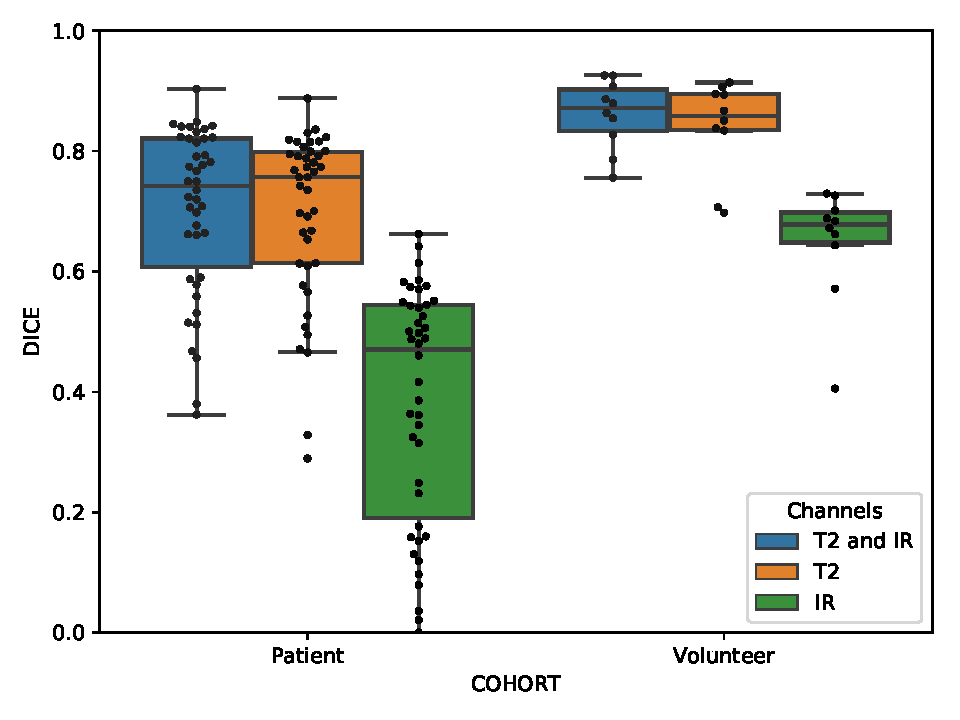
\includegraphics[width=0.8\textwidth]{boxplot_T2_IR_DICE}
    \caption[Boxplot for the \acrlong{dice} for the Baseline trained on T2 and IR separately.]{Boxplot for the \acrlong{dice} for the baseline architecture trained on both, T2 and IR, images as well as trained on each image channel separately. Note that comparable segmentation performance is achieved by only incorporating the T2 image channel. Using only the IR channel, however, results in a significantly lower performance.}
    \label{fig:results_boxplot_T2_IR_dice}
\end{figure}

\section{Experiment 2: 3D Context} \label{sec:exp_3dcontext} % ==================================================
We successfully trained the neural networks with the proposed architectures, which allows them for more \gls{3d} context incorporation. The mean and \gls{sd} for the \acrlong{dice}, \acrlong{vs} and \acrlong{hd95} are summarized in the Table~\ref{tab:results_3d_context_small} together with the baseline results. The complete Table~\ref{tab:results_3d_context}, also featuring the \acrlong{avd} and \acrlong{hd}, can be found in the appendix. A boxplot for the \acrlong{dice} is shown in Figure~\ref{fig:results_boxplot_dice}. Figure~\ref{fig:results_heatmap_dice} features a heatmap, listing all the achieved \acrlong{dice} values on the patients and volunteers for all neural network architectures. Training took 15 and 22 hours on a NVIDIA Titan Xp for the stack-wise and patch-wise neural networks, respectively.

\begin{table}[htbp]
   \centering
   \caption[Metrics for the different Architectures]{Values for the \acrlong{dice}, \acrlong{vs} and \acrlong{hd95}. The results for all the metrics can be found in the Table~\ref{tab:results_3d_context} in the appendix.}
   \begin{tabular}{l*{6}{l}}
      \toprule
      Cohort	& Neural Network	& DICE				& VS				& HD95\\
      			&					&					&					& (mm)\\
      \midrule
      Patient   & Base  & $0.704 \pm 0.139$ & $0.882 \pm 0.098$ & $16.526 \pm 17.025$ \\
                & Stack\_3to1  & $0.749 \pm 0.139$ & $0.896 \pm 0.123$ & $\mathbf{10.807 \pm 13.393}$ \\
                & Stack\_5to1  & $\mathbf{0.765 \pm 0.123}$ & $\mathbf{0.898 \pm 0.110}$ & $12.418 \pm 19.104$ \\
                & Stack\_5to3  & $0.717 \pm 0.135$ & $0.883 \pm 0.105$ & $19.312 \pm 22.545$ \\
                & Stack\_Proj  & $0.712 \pm 0.136$ & $0.889 \pm 0.094$ & $19.878 \pm 21.613$ \\
                & Patch & $0.682 \pm 0.128$ & $0.876 \pm 0.101$ & $24.241 \pm 20.896$ \\                
      \midrule
      Volunteer & Base  & $0.861 \pm 0.057$ & $0.921 \pm 0.056$ & $1.644  \pm 2.321 $ \\
                & Stack\_3to1  & $0.860 \pm 0.073$ & $0.925 \pm 0.043$ & $2.260  \pm 2.336 $ \\
                & Stack\_5to1  & $\mathbf{0.878 \pm 0.048}$ & $\mathbf{0.928 \pm 0.048}$ & $1.537  \pm 1.784 $ \\
                & Stack\_5to3  & $0.855 \pm 0.052$ & $0.928 \pm 0.062$ & $\mathbf{1.350  \pm 1.365} $ \\                
                & Stack\_Proj  & $0.842 \pm 0.051$ & $0.917 \pm 0.067$ & $1.642  \pm 1.549 $ \\
                & Patch & $0.806 \pm 0.068$ & $0.888 \pm 0.085$ & $7.992  \pm 13.474$ \\
      \bottomrule
   \end{tabular}
   \label{tab:results_3d_context_small}
\end{table}

\begin{figure}[htbp]
	\centering
	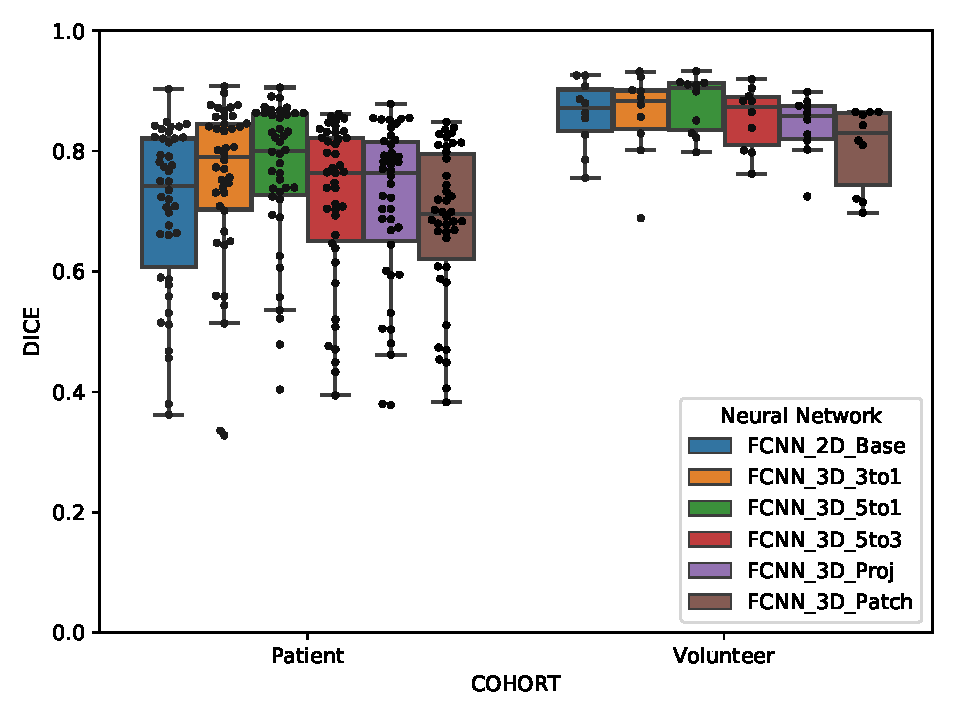
\includegraphics[width=\textwidth]{boxplot_DICE}
    \caption[Boxplot for the \acrlong{dice} of the different Architectures]{Boxplot for the \acrlong{dice} for the different neural network architectures.}
    \label{fig:results_boxplot_dice}
\end{figure}

\begin{figure}[htbp]	
	\centering
	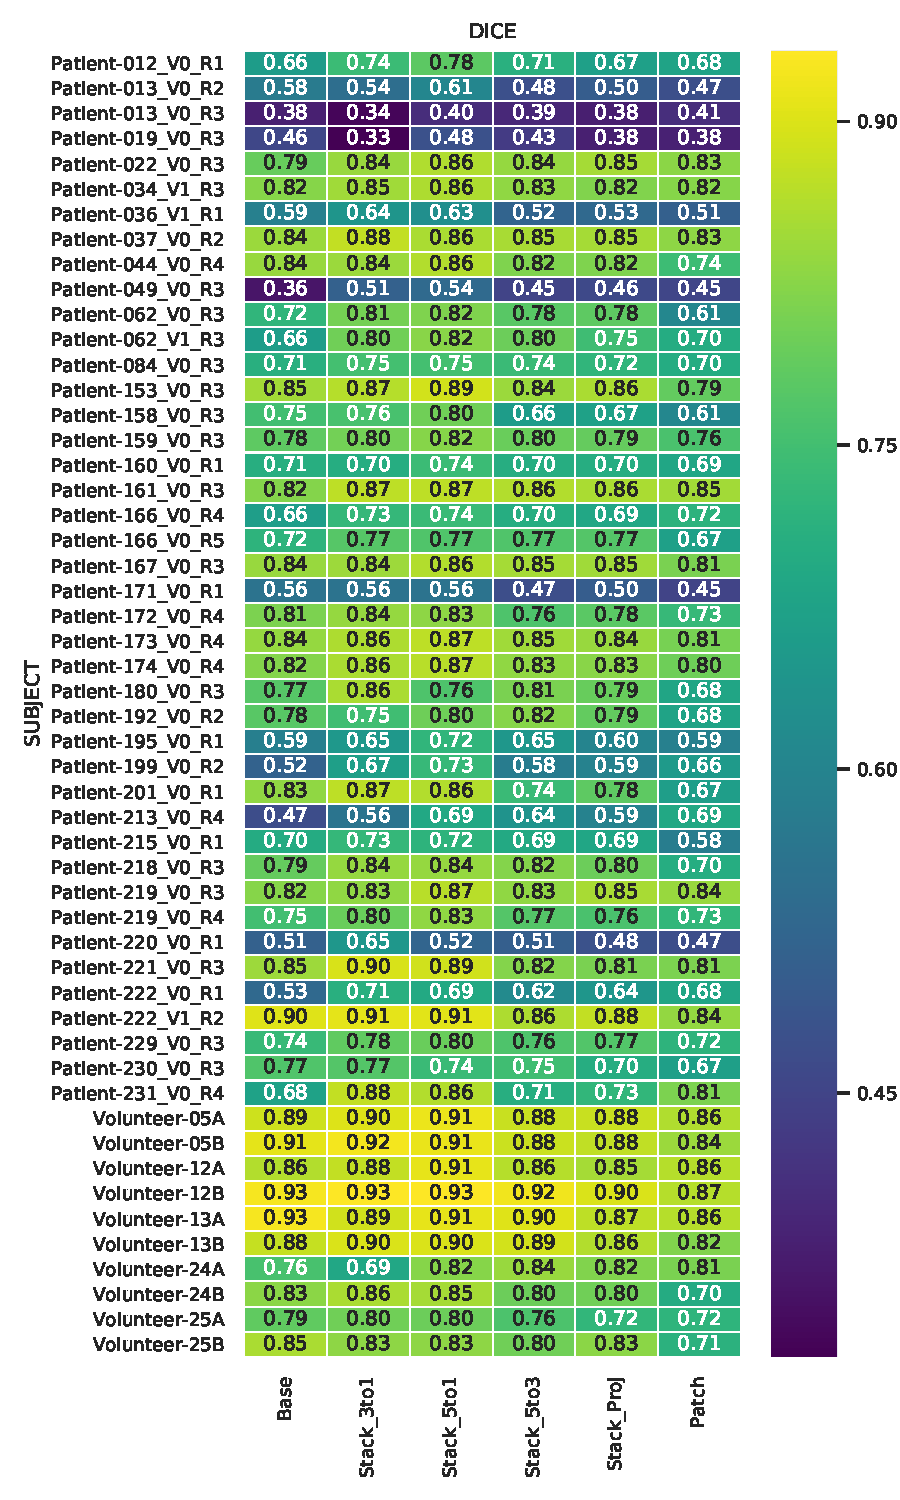
\includegraphics[width=\textwidth,height=\textheight,keepaspectratio]{heat_dice}
    \caption[Heatmap for the \acrlong{dice} of the different Architectures]{Heatmap for the achieved \acrlong{dice}s of the different neural network architectures.}
    \label{fig:results_heatmap_dice}
\end{figure}


\section{Experiment 3: Post-processing} \label{sec:exp_pp} % ====================================================
Table~\ref{tab:results_pp_small} presents the obtained results with respect to the \acrlong{dice}, \acrlong{vs} and \acrlong{hd95} metrics. The complete Table~\ref{tab:results_pp} can be found in the appendix. Figure~\ref{fig:pp_boxplots_hd95} shows the baseline and stack-wise architecture boxplot for the \acrlong{hd95}. The boxplots regarding the other metrics (Figures~\ref{fig:pp_boxplots_vs} to \ref{fig:pp_boxplots_hd}) are also situated in the appendix. We only show the boxplots for the \gls{hd95} here because the overlap-based metrics are not influenced to much by the post-procssing.
Post-processing was done on a desktop PC with a 6-core Intel i7 processor, and took 3 minutes for keeping the $n$ largest volumes only (\textit{Volumes only}) for all 52 subjects. The number of volumes to keep was tuned for both architectures, resulting in $n = 3$ and $n = 2$ volumes for the baseline and stack-wise architecture, respectively. Joining the volumes and then keeping only the largest one (\textit{Joint volumes}) took one hour to process for all 52 subjects.



\begin{figure}[htbp]
	\centering
	\subfloat[]
	{
		\label{fig:subfig:pp_base_219}
		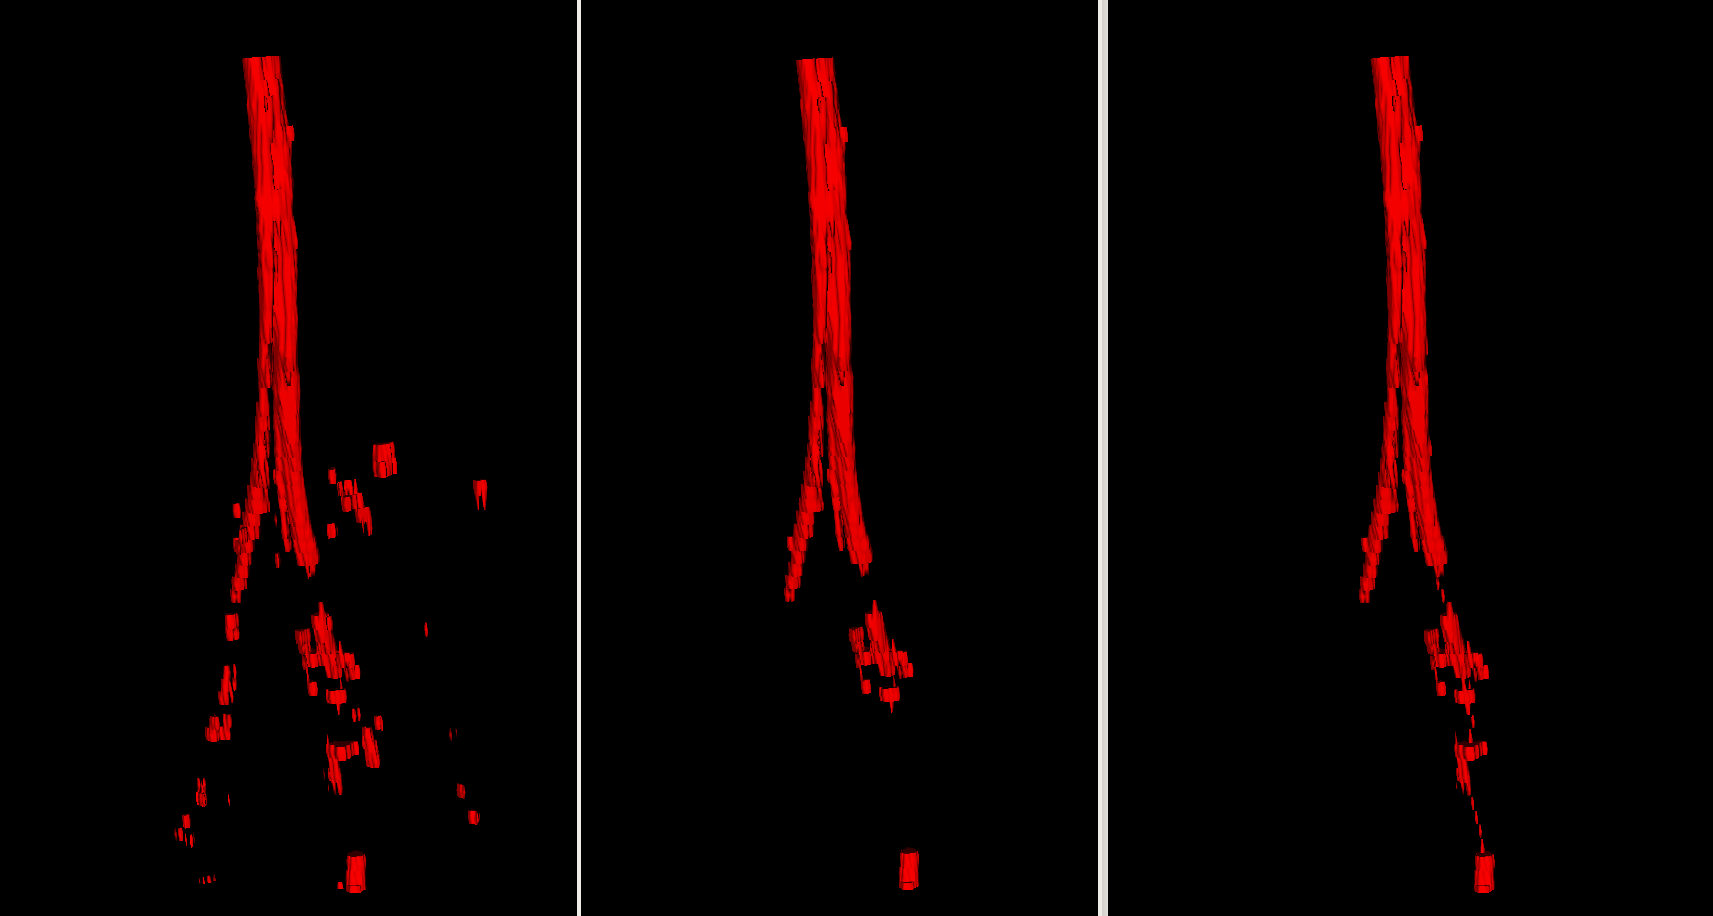
\includegraphics[width=\textwidth]{pp_base_219}
	}
	\hfill
	\subfloat[]
	{
		\label{fig:subfig:pp_5to1_219}
		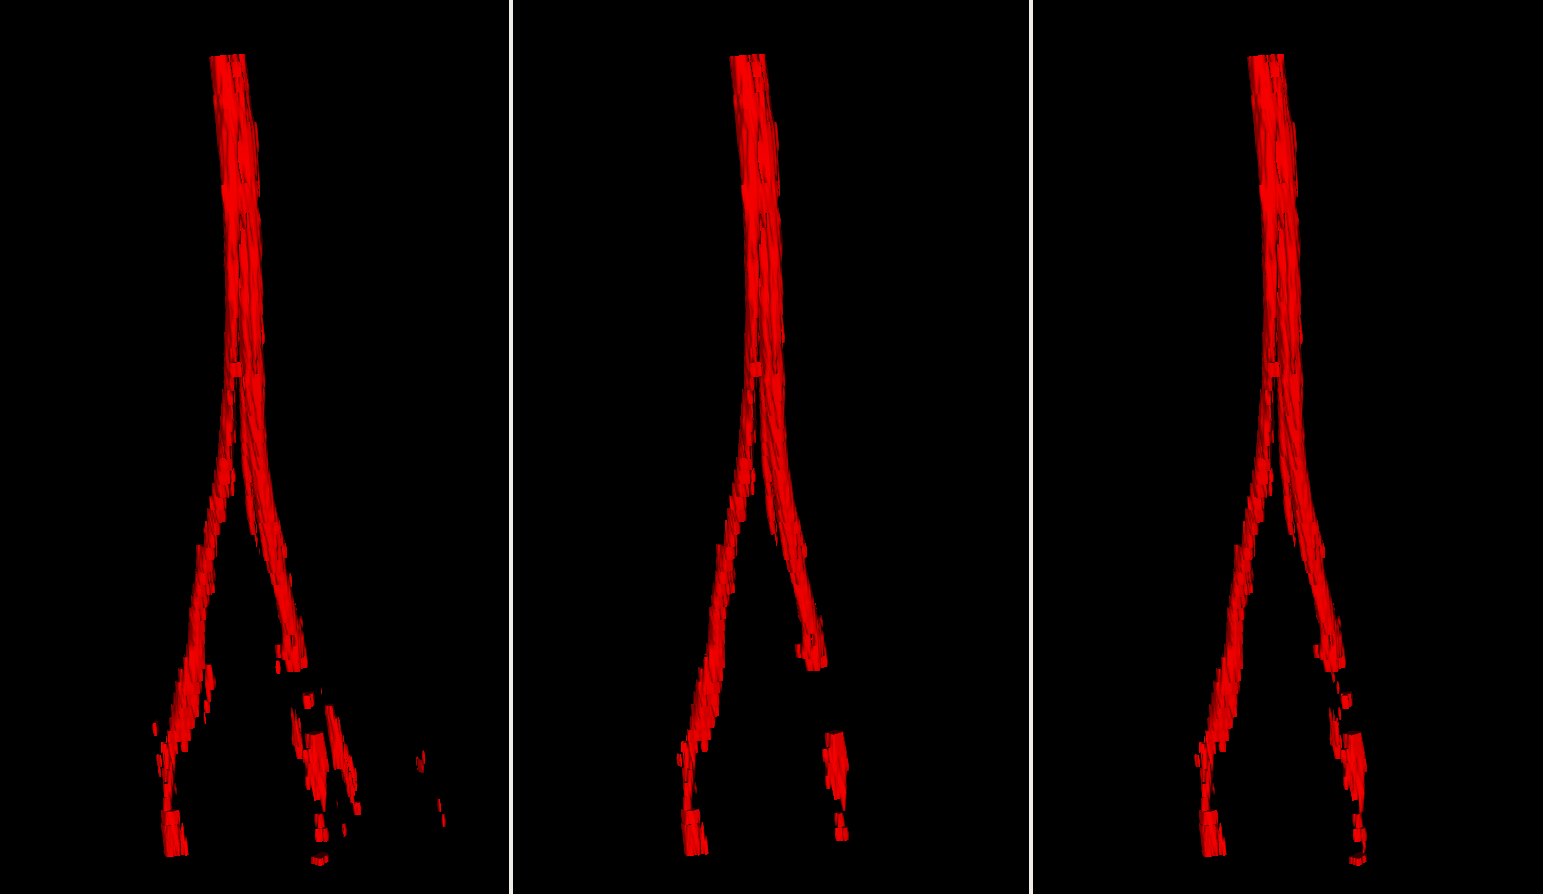
\includegraphics[width=\textwidth]{pp_5to1_219}
	}
	\caption[Post-processing impact on Base and Stack]{\gls{3d} segmentation renderings of a patient's sciatic nerve. \textbf{a)} Output segmentation of the baseline without post-processing (left), with $n$ largest volumes only (center) and with full post-processing (right). \textbf{b)} Output segmentation of the best performing stack-wise architecture without post-processing (left), with $n$ largest volumes only (center) and with full post-processing (right).}
	\label{fig:pp_patient_219}  
\end{figure}


\begin{table}[htbp]
   \centering
   \caption[Segmentation Evaluation Metrics for the different Architectures]{Values for the \acrlong{dice}, \acrlong{vs} and \acrlong{hd95} for the baseline and stack architecture. \textit{Volumes only} means that only the $n$ largest volumes were kept ($n = 3$ and $n = 2$ for the Base and Stack\_5to1 architecture, respectively). \textit{Joint volumes} means that we tried to connect the correctly segmented volumes first, and then only kept the largest one.}
   \begin{tabular}{l*{7}{l}}
      \toprule
      Cohort	& Network	& Post-processing	& DICE				& VS				& HD95\\
      			&					&					&					&					& (mm)\\
      \midrule
      Patient   & Base 	& None & $0.705 \pm 0.137$ & $\mathbf{0.883 \pm 0.097}$ & $16.285 \pm 16.896$\\
                &                	& Volumes only  & $0.711 \pm 0.145$ & $0.867 \pm 0.125$ & $20.364 \pm 20.125$\\
                &                	& Joint volumes & $\mathbf{0.722 \pm 0.136}$ & $0.873 \pm 0.125$ & $\mathbf{11.812 \pm 12.785}$\\
      \midrule
      Patient   & Stack\_5to1 	& None & $0.765 \pm 0.123$ & $0.898 \pm 0.110$ & $12.418 \pm 19.104$\\
                &                	& Volumes only  & $0.772 \pm 0.120$ & $0.899 \pm 0.119$ & $11.481 \pm 16.706$\\
                &                	& Joint volumes      & $\mathbf{0.779 \pm 0.123}$ & $\mathbf{0.905 \pm 0.117}$ & $\mathbf{6.688  \pm 10.332}$\\
      \midrule
      Volunteer & Base 	& None & $0.861 \pm 0.057$ & $0.921 \pm 0.056$ & $1.644  \pm 2.321 $\\
                &                	& Volumes only  & $0.862 \pm 0.057$ & $0.924 \pm 0.056$ & $2.311  \pm 4.508 $\\
                &                	& Joint volumes      & $\mathbf{0.868 \pm 0.050}$ & $\mathbf{0.929 \pm 0.056}$ & $\mathbf{1.230  \pm 1.255}$\\
      \midrule
      Volunteer & Stack\_5to1 	& None & $0.884 \pm 0.046$ & $0.927 \pm 0.051$ & $1.140  \pm 1.344 $\\
                &                	& Volumes only  & $0.883 \pm 0.046$ & $0.933 \pm 0.049$ & $1.357  \pm 1.454 $\\
                &                	& Joint volumes      & $\mathbf{0.894 \pm 0.042}$ & $\mathbf{0.942 \pm 0.050}$ & $\mathbf{0.655  \pm 0.355}$\\
      \bottomrule
   \end{tabular}
   \label{tab:results_pp_small}
\end{table}

\begin{figure}[htbp]
	\centering
	\subfloat[]
	{
		\label{fig:subfig:pp_boxplot_base_hd95}
		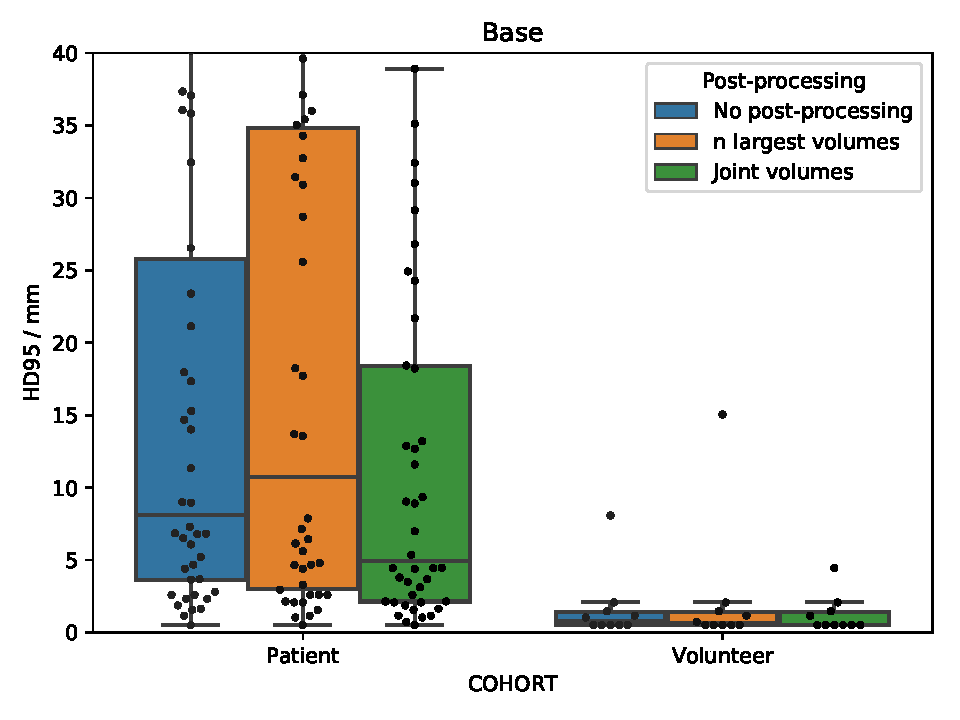
\includegraphics[width=0.7\textwidth]{pp_boxplot_base_HD95}
	}
	\hfill
	\subfloat[]
	{
		\label{fig:subfig:pp_boxplot_5to1_hd95}
		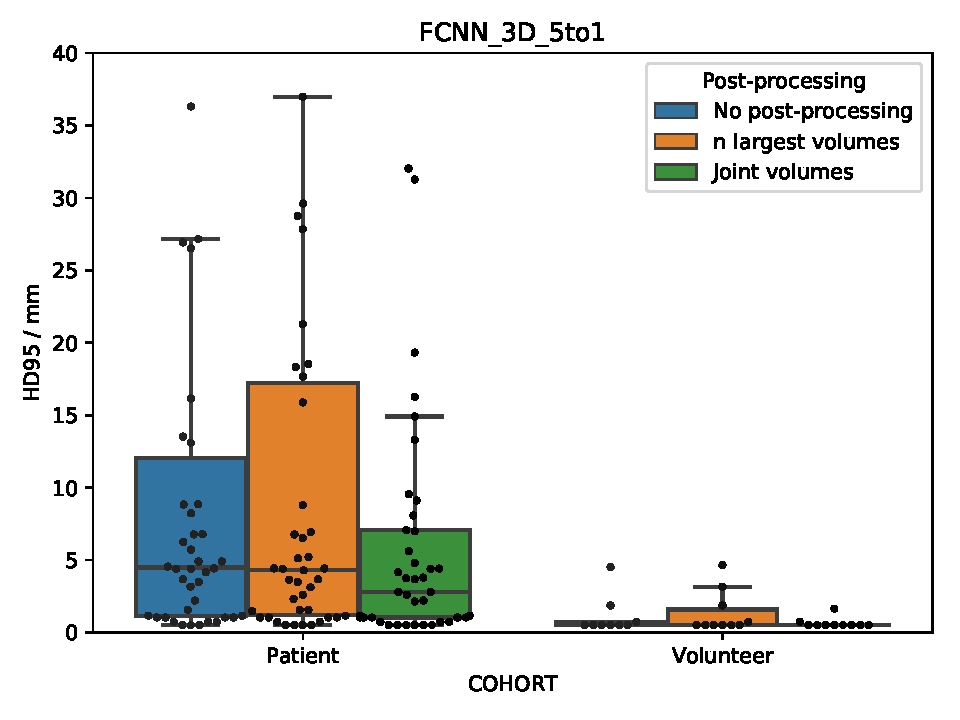
\includegraphics[width=0.7\textwidth]{pp_boxplot_5to1_HD95}
	}
	\caption[Post-processing impact on \acrlong{hd95}]{Boxplots for the \acrlong{hd95} for the \textbf{a)} baseline and best performing \textbf{b)} stack-wise architecture. \textit{n largest volumes} means that only the $n$ largest volumes were kept ($n = 3$ and $n = 2$ for the base and Stack\_5to1 architecture, respectively). \textit{Joint volumes} means that we tried to connect the correctly segmented volumes first, and then only kept the largest one.}
	\label{fig:pp_boxplots_hd95}  
\end{figure}





\section{Evaluation} \label{sec:exp_evaluation} % ===============================================================
In Figure~\ref{fig:res_inter_rater} the inter-rater variability is shown for all the rater-rater combinations and metrics. Table~\ref{tab:results_durations} contains all the different times required for the individual steps involved in the peripheral nerve segmentation.

\begin{figure}[htbp]	
	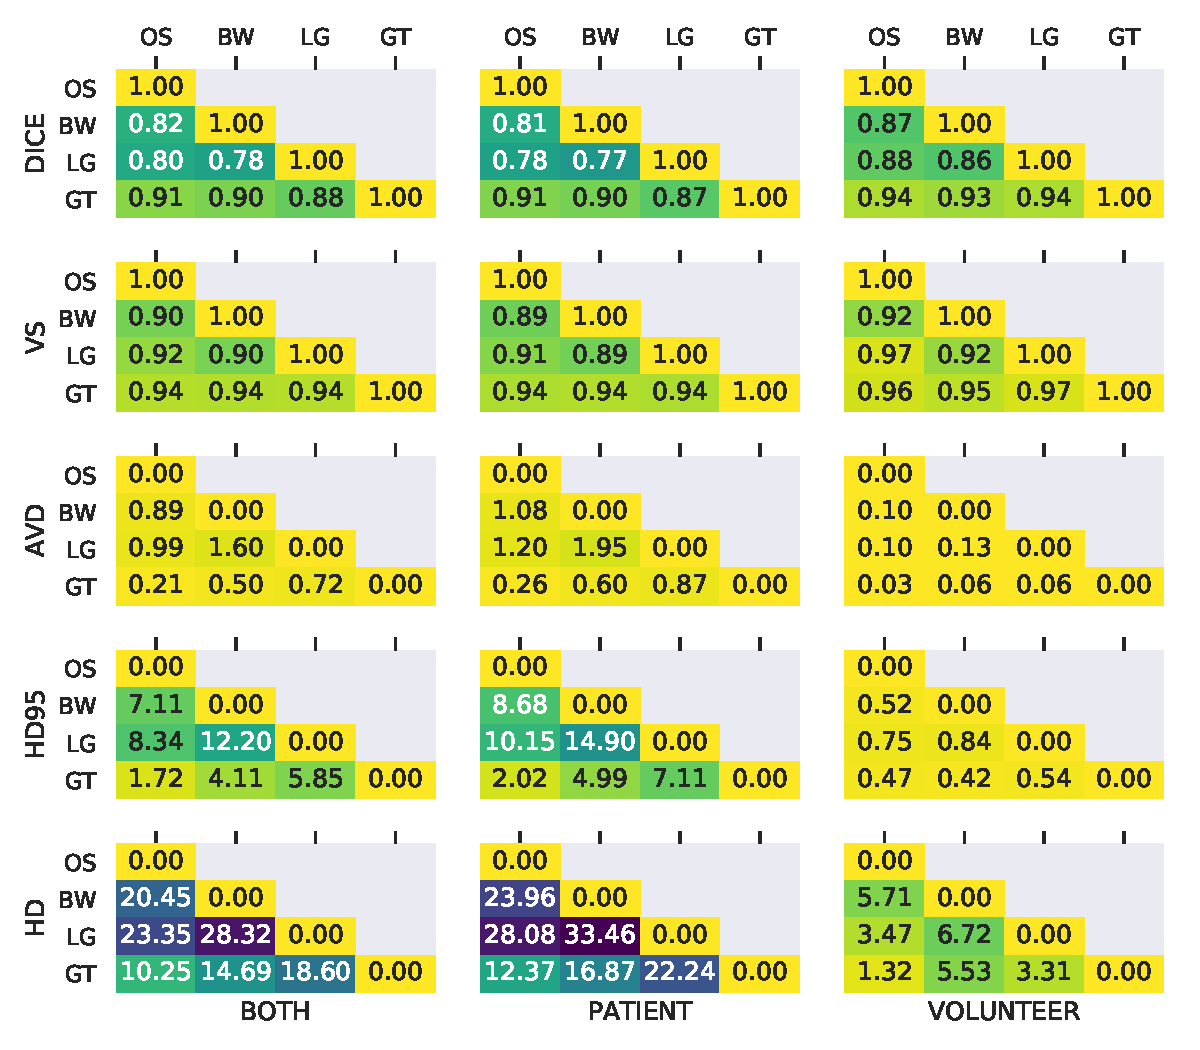
\includegraphics[width=\textwidth]{inter_rater}
    \caption[Inter-Rater Agreement]{Inter-rater agreement for the \acrlong{dice}, \acrlong{vs}, \acrlong{avd}, \acrlong{hd95} and \acrlong{hd} per cohort. Values close to 1.00 for \gls{dice} and \gls{vs} correspond to a high level of agreement between the raters. Conversely, low values for \gls{avd}, \gls{hd95} and \gls{hd} imply higher agreement.}
    \label{fig:res_inter_rater}
\end{figure}


\begin{table}[htbp]
   \centering
   \caption[Time Requirements]{Time requirements for the different steps involved in the peripheral nerver segmentation. All the durations for pre-processing, evaluation and post-processing are given as the time required to process a single \gls{mrn} case.}
   \begin{tabular}{l*{6}{l}}
      \toprule
      Phase	        & Step                  & Variant               & Duration\\
      \midrule
      Training      & Training              & Base                  & 2 h   \\
                    &                       & Stack (all)           & 15 h  \\
                    &                       & Patch                 & 22 h  \\
      \midrule
      Pre-processing& Registration          &                       & $1 \pm 0.5$ m \\
      \midrule
      Evaluation    & Segmentation          &                       & 3 s \\
                    & Post-processing       & $n$ largest volumes   & 4 s \\
                    &                       & Joint volumes         & 1 m \\
      \midrule
      Fully automatic segmentation & & & 2 $\pm$ 0.5 m\\
      (After training, full Post-processing)\\
      \midrule
      Manual ground truth segmentation & & & $24 \pm 8$ m\\
      (done by expert) \\
      \bottomrule
   \end{tabular}
   \label{tab:results_durations}
\end{table}





\endinput